\chapter{Raster formatting}

Visualizing raster data requires an understanding of how it works from a technical perspective.

\section{Bit depth} 
Common raster formats include jpeg, png and tiff. One of the key differences between these formats are the bit depth. This value determines how many different colors that can be assigned to each pixel in the image. Each bit can only be assigned one of two values, 0 or 1. This number of available colors for a pixel can therefore be calculated as $2^{\:number\: of\: bits}$. As an example, a bit depth of 8 bits would then result in $2^8 = 256$ different potential colors, since this is the number of combinations of ones and zeroes, that are possible. For most maps this amount of colors is enough. The human eye can comprehend around 10 million different colors, but often that many colors are not needed. When displaying aerial photographs, the depth of 24 bits is often used, since it can display 16.7 million different colors. The human eye is able to perceive around 10 million colors, so this bit depth can therefore appear in true-colors to humans.
The limitations of the human eye does not mean that having more than 10 million bit combination is pointless. The bit combination can also be used for other thing than colors. It can be used to create transparency values or to store metadata about the image file. For instance, the geotiff format can use the additional bit to store georeferencing information.
These advantages of higher bit count come at a cost of a larger file size. Having a larger color depth will result in a slower loading and larger requirements for storage space. \citep{Dent} %Dent. 283 

\section{Tiled raster}
This section describes standards for dividing large raster files into smaller tiles. 
A way of only visualising the necessary parts of a raster is to divide it into smaller raster tiles and then only load the relevant tiles. When loaded into the map these tiles then get places next to each other, so they appear as a single large map image. These tiles can also be created with different resolutions, so that zooming in on the map with return tiles higher spatial resolution.  As illustrated in figure \ref{TilesPerZoomLevel} each of these zoom layers have more tiles.
\citep{Liedman}
When zoomed all the way out the entire world is rendered as a single tile. Whenever the zoom level gets increased by one each tile in the previous layer get replaced with four smaller tiles. The number of tiles on a zoom level z can therefore be calculated as $2^{2z}$.
\citep{SlippyMap}

\begin{figure} [H]
	\centering
	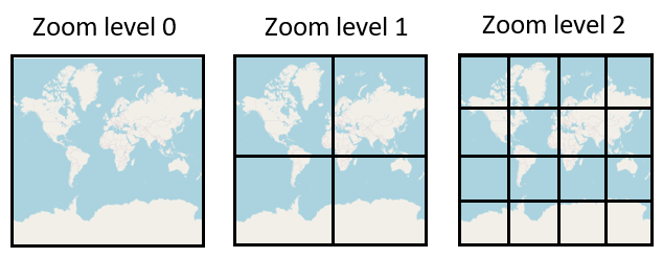
\includegraphics[width=.8\textwidth]{Pictures/TilesPerZoomLevel}
	\caption{Illustration of the increase in tiles for each zoom level}
	\label{TilesPerZoomLevel}
\end{figure}

Openstreetmaps is an example of a service, which use tiled rasters for their map. When this service is used, requests for tiles are send to 
http://tile.openstreetmap.org/zoom/x/y.png
In the request the values zoom, x and y are replaced with the current zoom level, tile column and tile row.
\citep{SlippyMap}


The naming of these tiles are done differently for different standards. In this section only the Tile Map Service (TMS) and Slippy map (XYZ) standard will be addressed. Both of these have the same approach to naming zoom level and columns, but different approach to naming the rows. This difference has been illustrated in figure \ref{TMSXYZ}. The reason for the difference is that TMS tiles number their rows from south northwards, whereas XYZ are numbering rows the reverse way. %Due to this difference in numbering rows loading tiles from the wrong standard results in a map as shown in figure \ref{SlippyInTMS}.
\citep{TMS}

\begin{figure} [H]
	\centering
	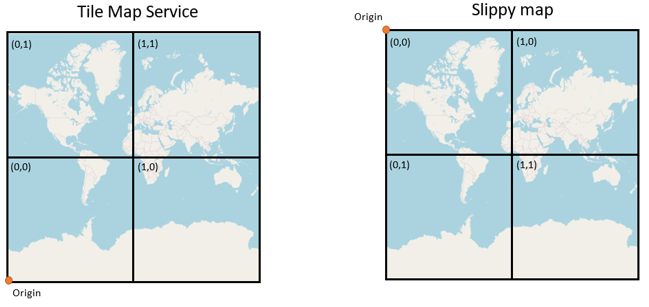
\includegraphics[width=.8\textwidth]{Pictures/TMSXYZ}
	\caption{Illustration of the difference between the TMS and XYZ formats. The individual maps are inspired similar maps from \citet{Slippy101} and \citet{TMSnaming}}
	\label{TMSXYZ}
\end{figure}

%
%\begin{figure} [H]
%	\centering
%	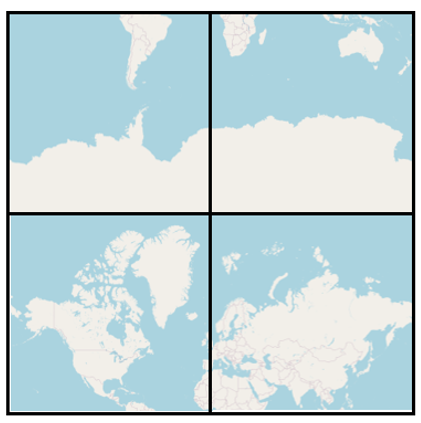
\includegraphics[width=.3\textwidth]{Pictures/SlippyInTMS}
%	\caption{How the map looks, when the TSM and XYZ get switched}
%	\label{SlippyInTMS}
%\end{figure}